\documentclass[9pt,twocolumn,twoside]{pnas-report}

\templatetype{pnasresearcharticle}

\usepackage{lipsum}

% set figures directory to be ./figures
\graphicspath{{./figures/}}

\title{Draft}

\author[a]{Žiga Trček}
\author[a]{Matej Urbas}
\author[a]{Jan Vasiljević}

\affil[a]{University of Ljubljana, Faculty of Computer and Information Science, Ve\v{c}na pot 113, SI-1000 Ljubljana, Slovenia}

\leadauthor{Jan Vasiljević}

\authordeclaration{All authors contributed equally to this work.}
\correspondingauthor{\textsuperscript{1}To whom correspondence should be addressed. E-mail: fine.author@email.com.}

\begin{abstract}
We study a phenomenon that we claim is important in a subject in which we claim many people are interested. We also claim that such ideas have been studied heavily both in network science and in other disciplines, although all prior work on this topic is horrible (though we will try to phrase that statement as politely as possible). One particular idea, which has some intriguing features but which either rarely has been studied or has only been studied in a crappy way before, is the one that we investigate in this project. Invoking minimal sarcasm, we study an extended version of this idea with our new approach, which we will claim to give universal results if we can get away with it. Our new approach has some bells and whistles that we study in our project, and we use computations, theory, and experiments to give important insights into a phenomenon that many people care about. We also give some gratuitous caveats so that peers will take us seriously, and we pray to our favorite deity that this approach is not equivalent to one that already exists (we forgot to check, but the authors need to graduate). We hope that our study, in addition to its intrinsic quality, will inspire future investigations, citations, and successful grants (and --- who knows? --- maybe even a Turing Award). In case you did not see it last time, we claim once again that our approach is universal.
\end{abstract}

\dates{The manuscript was compiled on \today}
\doi{\href{https://ucilnica.fri.uni-lj.si/course/view.php?id=183}{Introduction to Network Analysis} 2023/24}

\begin{document}

\maketitle
\thispagestyle{firststyle}
\ifthenelse{\boolean{shortarticle}}{\ifthenelse{\boolean{singlecolumn}}{\abscontentformatted}{\abscontent}}{}

\dropcap{P}{\bf roblem definition, motivation, background, contributions etc.}
\lipsum[1-4]

\begin{figure}[t]\centering%
	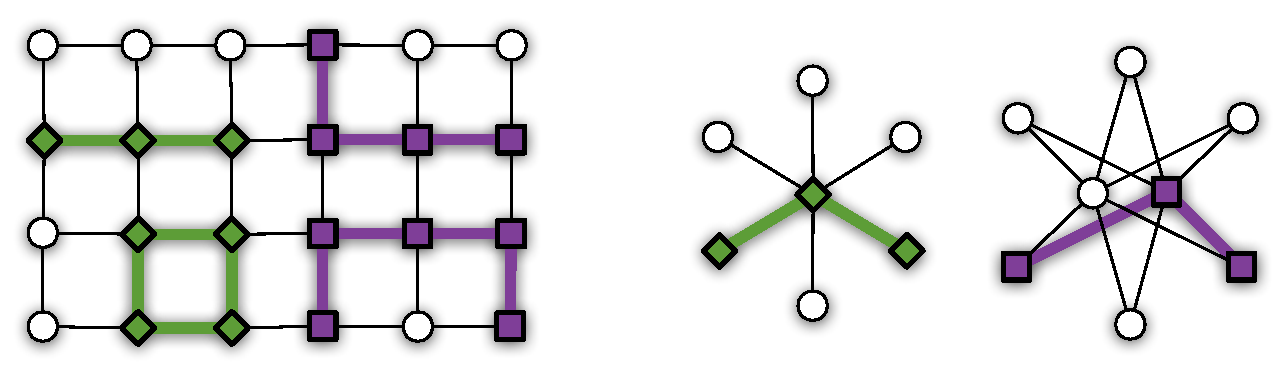
\includegraphics[width=0.9\linewidth]{examples}
	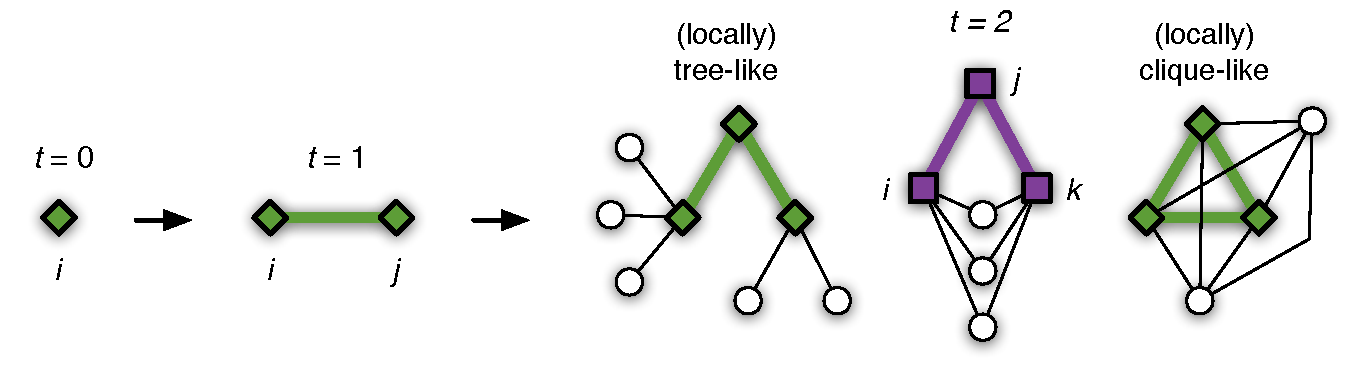
\includegraphics[width=\linewidth]{growth}
	\caption{Mandatory informative illustration highlighting main contributions.~\cite{Sub18a}}
	\label{fig:example}
\end{figure}

\section*{Related work}

{\bf Relevant literature ($\approx 10$ references).}
\lipsum[5-6]

\nocite{Kle00,Bou05,EB07,New08,For10,New12,FH16,PLC17,PDL18,Pei20}

\section*{Results}

{\bf Main results supported by math, plots, tables, diagrams etc.}
\lipsum[1]

\begin{table}[h]\centering%
	\caption{Table describing data or methods.}
	\begin{tabular}{lccccc}\toprule
	    & $n$ & $m$ & $\langle k\rangle$ & $\langle C\rangle$ & $\langle d\rangle$ \\\midrule
	    Fine network & $438\,920$ & $9\,742\,733$ & $44.4$ & $0.37$ & $6.19$ \\
	    Random graph & $438\,920$ & $9\,781\,609$ & $44.6$ & $0.00$ & $4.92$ \\\bottomrule
	\end{tabular}
	\label{tbl:example}
\end{table}

\lipsum[2-3]

\begin{figure}[t]\centering%
	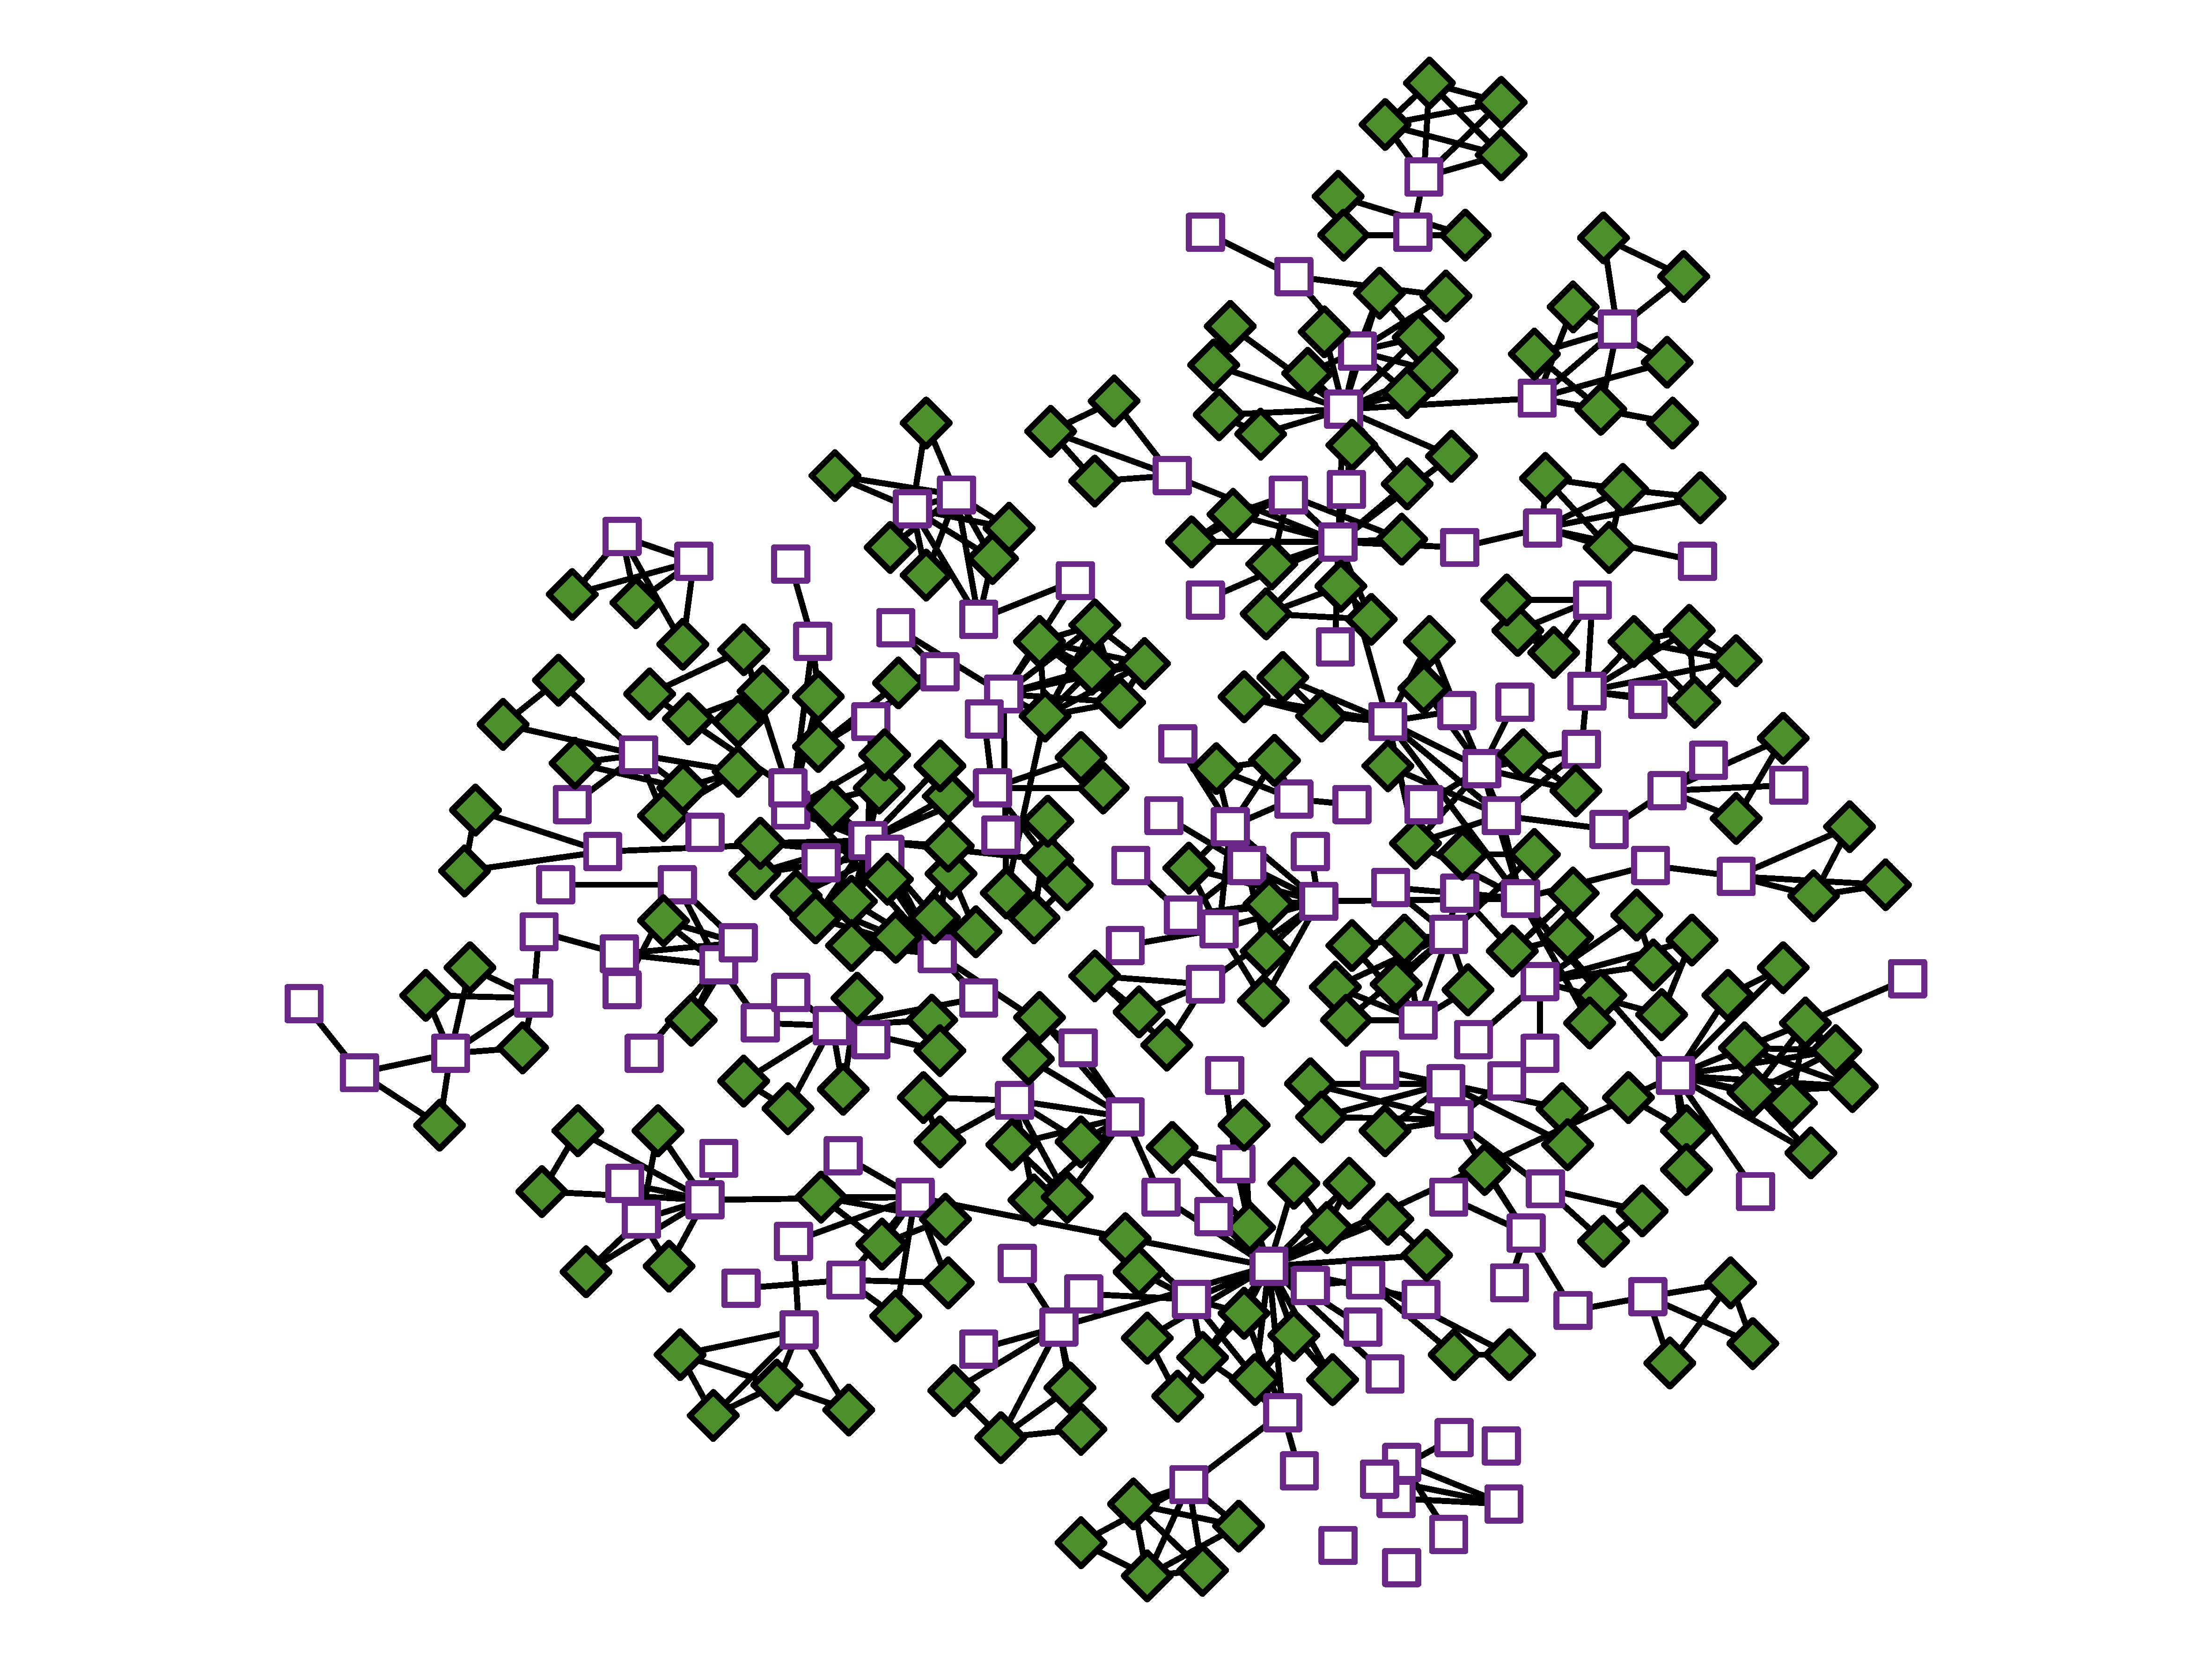
\includegraphics[width=0.49\linewidth]{example1}
	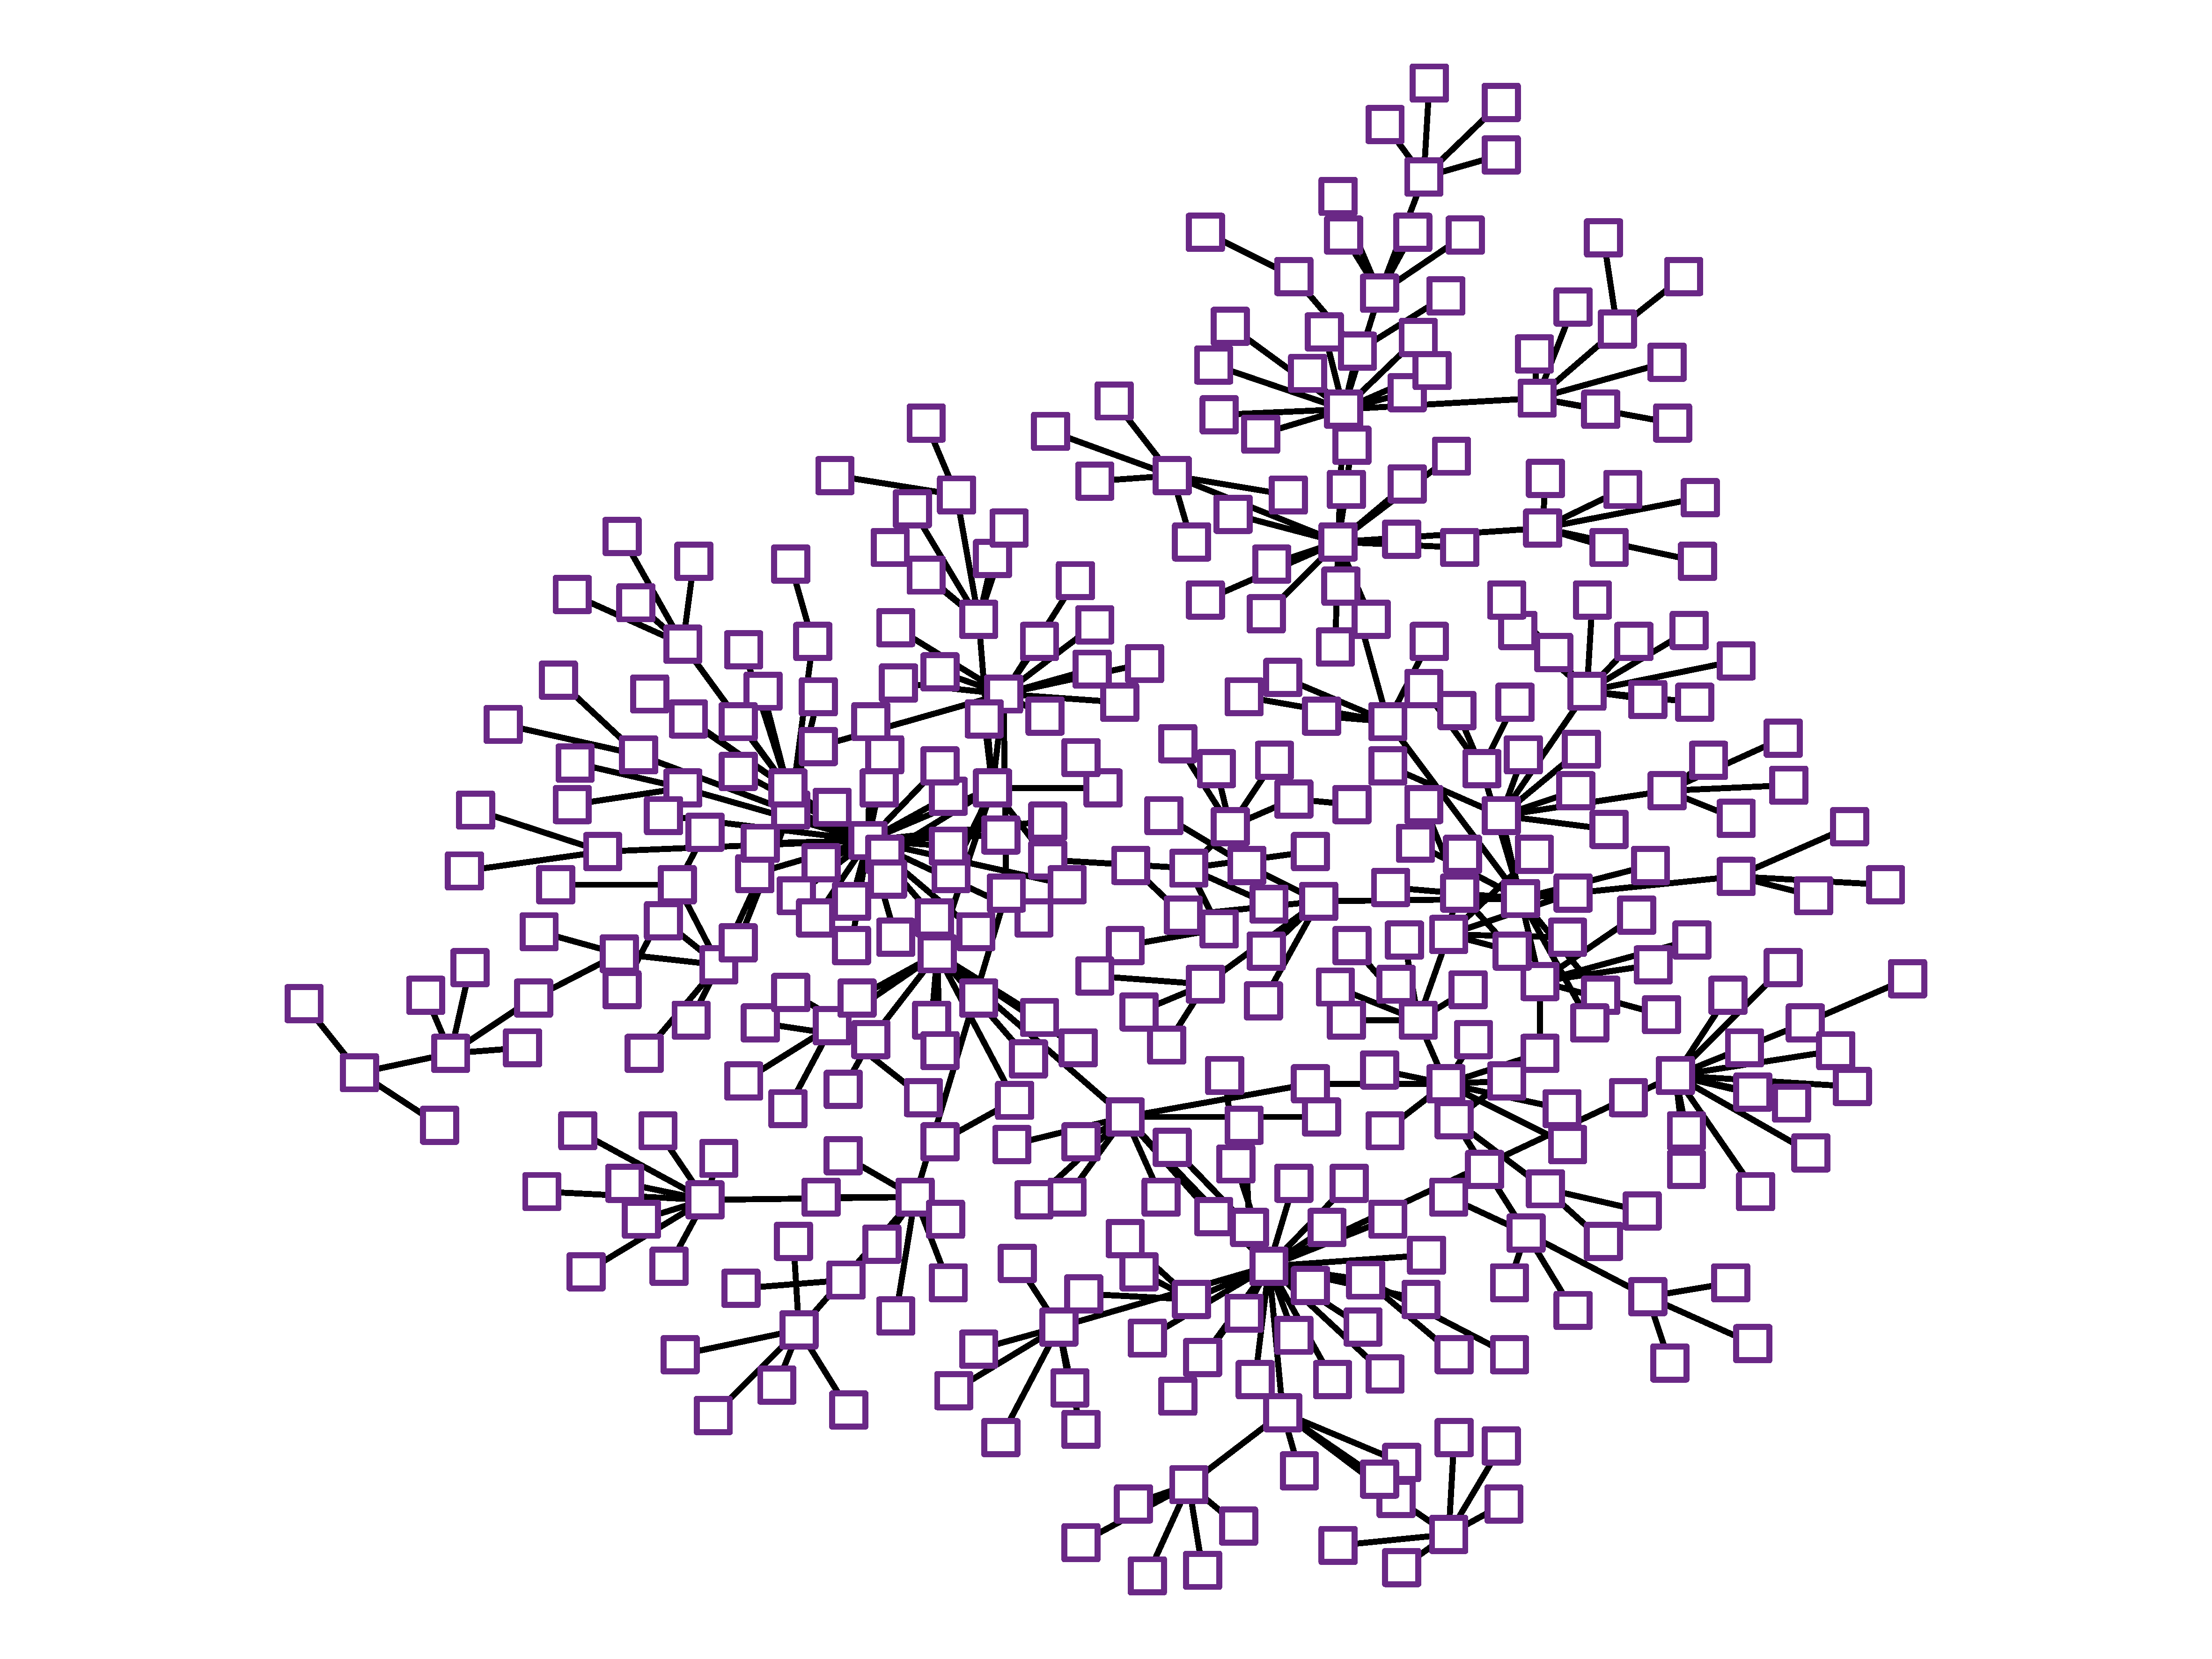
\includegraphics[width=0.49\linewidth]{example2}
	\caption{Figure showing interesting examples.~\cite{Sub18a}}
\end{figure}

\lipsum[4-6]

\begin{figure}[b]\centering%
	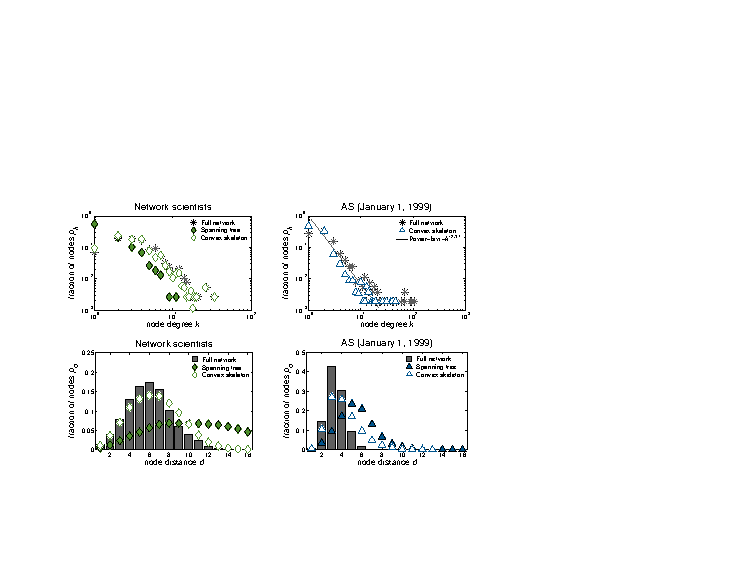
\includegraphics[width=\linewidth]{distributions}
	\caption{Figure showing relevant results.~\cite{Sub18a}}
\end{figure}

\begin{figure}[t]\centering%
	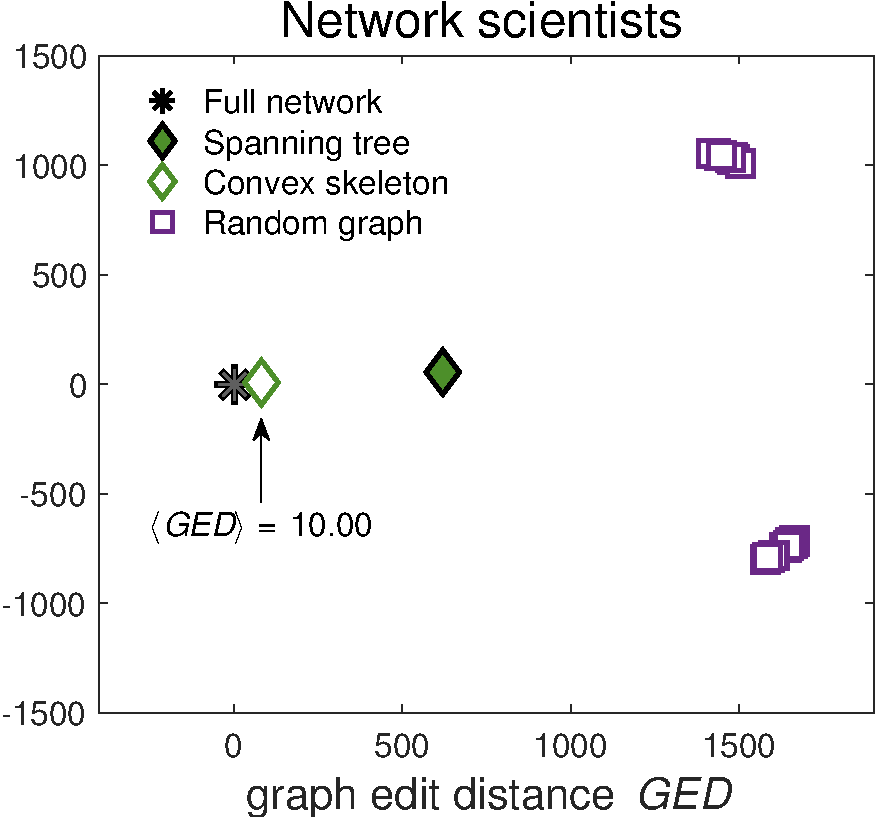
\includegraphics[width=0.45\linewidth]{results1}\hskip12pt
	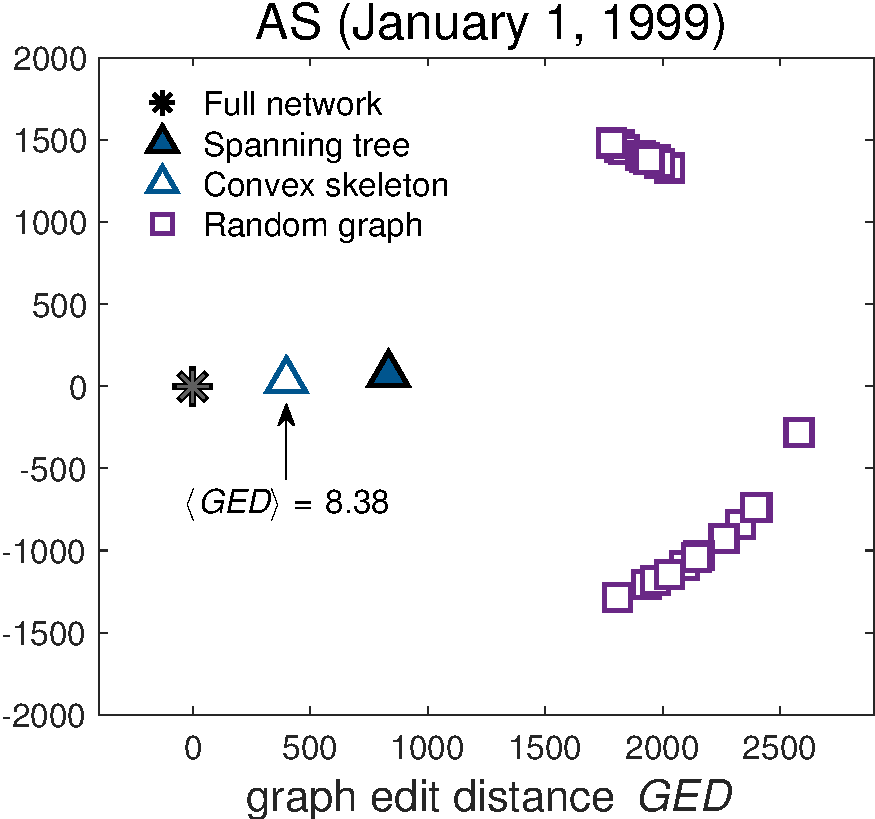
\includegraphics[width=0.45\linewidth]{results2}
	\caption{Another figure with results.~\cite{Sub18a}}
	\label{fig:example}
\end{figure}

\section*{Discussion}

{\bf Summary of results, main contributions, final conclusions, future work etc.}
\lipsum[1-3]

{\small

\section*{Methods}

{\bf Data, methods, algorithms etc.}
\lipsum[1]

\begin{equation}
	\phi_v = \Pr(X_{st}(v) = 1) = \Pr(X_{sv} = 1)\Pr(X_{vt} = 1)
	\label{eq:example}
\end{equation}

\lipsum[2]

\begin{algorithm}[H]
	\begin{algorithmic}[1]
		\Require graph $G$, cutoff $k_{min}$
		\Ensure power-law $\gamma$ 
		\State $s\gets$ $n\gets$ $0$
		\For{nodes $i\in N$} 
			\If {$k_i\geq k_{min}$}
				\State $s\gets$ $s+\ln k_i/(k_{min}-0.5)$
				\State $n\gets$ $n+1$
			\EndIf
		\EndFor
		\State \Return $1+ns^{-1}$
	\end{algorithmic} \vspace{8pt}
\end{algorithm}

\lipsum[3-4]

}

% \acknow{The authors would like to\dots}

% \showacknow{}

\bibliography{bibliography}

\end{document}